% SPDX-License-Identifier: Apache-2.0
%
% The report on the wdbcvt effort. Built by //docs/latex:report through
% rules_latex_host, which calls the host pdflatex three times.
\documentclass[conference]{IEEEtran}

\usepackage{booktabs}
\usepackage{graphicx}
\usepackage{url}
\usepackage{listings}
\usepackage{xcolor}
\usepackage{balance}

\lstset{
  basicstyle=\ttfamily\scriptsize,
  columns=fullflexible,
  breaklines=true,
  frame=single,
  framesep=3pt,
  captionpos=b,
  keepspaces=true,
}

\begin{document}

\title{Reading an Undocumented Waveform Database:\\
A Differential Corpus Method, Applied to Vivado \texttt{xsim}}

\author{\IEEEauthorblockN{An automated coding assistant}
\IEEEauthorblockA{HDL Factory\\
Report generated from the \texttt{wdbcvt} repository\\
\url{https://git.hdlfactory.com/HDL/wdbcvt}}}

\maketitle

\begin{abstract}
AMD Vivado's \texttt{xsim} simulator records a run into a
\texttt{.wdb} waveform database that no other tool reads, and the VCD
file it writes from the same run holds only part of the design: for
eight of the fifteen VHDL types in our test corpus the VCD contains no
variable declaration at all. This report describes how the container,
the type table, the hierarchy and the value records of that database
were worked out without documentation, source or a decompiler, using a
corpus of 1061 minimal test cases in which each case differs from
another in one way, and a ground truth file per case written from the
design rather than from the database. It states the resulting reader,
its output path to FST through the reference library \texttt{libfst},
and the measurements over six designs, the largest of which is a dual
core RISC-V system on chip with 5696 recorded objects and 18\,875\,466
value changes. It also states the limits: every claim is scoped to
Vivado 2025.2, the derivation was performed by an AI agent under human
supervision, and the result is not a specification.
\end{abstract}

\begin{IEEEkeywords}
waveform database, VCD, FST, file format analysis, hardware
simulation, differential testing, Bazel
\end{IEEEkeywords}

% SPDX-License-Identifier: Apache-2.0
\section{Introduction}

A simulation run under AMD Vivado's \texttt{xsim} writes two files. The
waveform database, \texttt{sim.wdb}, holds every signal the simulator
was told to record. The value change dump, \texttt{sim.vcd}, holds a
subset in the text format defined by IEEE~1800~\cite{ieee1800}.

The subset is smaller than it appears. Measured across the corpus
described in this report, Vivado's own VCD omits, for eight of the
fifteen VHDL types present, both the variable declaration and every
value change. Absent are \texttt{boolean}, \texttt{integer},
\texttt{real}, \texttt{time}, \texttt{character}, user enumerations,
records and arrays. Present are \texttt{std\_ulogic}, \texttt{bit} and
their vector types. A tool that reads the VCD therefore sees a design
with most of its state removed, and nothing in the file says so.

The database that does hold the state is undocumented, and until now
no tool outside Vivado read it. This report describes:

\begin{itemize}
  \item a method for working out such a format from experiments, based
        on a corpus of minimal pairs and a declared ground truth per
        case (Section~\ref{sec:method});
  \item what that method established about the \texttt{.wdb}
        container, its type table, its hierarchy and its value records
        (Section~\ref{sec:format});
  \item how the result is guarded against the failure mode particular
        to a derivation of this kind, namely a plausible story that
        happens to reproduce (Section~\ref{sec:validation});
  \item a converter to FST~\cite{fst}, a format that can hold what the
        database holds, written through the reference implementation
        rather than reimplemented, and to SQLite for the reader that
        queries rather than looks (Section~\ref{sec:output});
  \item the limits of all of it (Section~\ref{sec:limitations}).
\end{itemize}

The work was performed by an AI agent under human supervision. That
fact is stated in the repository's README, in its provenance document
and in the tool's \texttt{-{}-help} output, and it is repeated here
because it changes how the result should be read: an agent that infers
a format from examples produces measurements that reproduce and
plausible stories about bytes, and the two are indistinguishable on
the page. The method in Section~\ref{sec:method} exists to separate
them.

The subject is Vivado 2025.2. No other version has been observed, and
no claim here should be assumed to hold for one.

% SPDX-License-Identifier: Apache-2.0
\section{Method}
\label{sec:method}

\subsection{Minimal pairs}

The corpus is a set of small designs, each simulated once, each
differing from another case in exactly one property. A finding is the
difference between the two databases that results.

Two examples. \texttt{t10\_vec274} declares a value of 274 bytes and
\texttt{t10\_vec275} declares 275; the first is written as one record
and the second as two, which locates the threshold at which a large
value is split into chunks. \texttt{t2\_bit} and
\texttt{t1\_bit\_one\_edge} differ in the type of a single signal, and
the difference between the two type tables is the entry that
distinguishes \texttt{BIT} from \texttt{STD\_ULOGIC}.

Cases are grouped into tiers, each tier asking one question. The
corpus reached 1146 cases in 79 tiers. Each case directory holds the
source, a \texttt{BUILD.bazel} that simulates it, and a
\texttt{truth.json}.

\subsection{Ground truth declared before the file is opened}

\texttt{truth.json} states what the simulation must produce: the
signals with their scopes, widths and type names, the value of each at
each time, and, where a tier needs it, the number of raw records a
signal holds. It is derived from the design source. It is not derived
from the database, and it is written before the database is decoded.

This is what makes a decoding claim falsifiable. The reader must
reproduce the truth file; a decoding that merely reproduces itself
fails.

\subsection{The noise mask}

Not every byte of a database is a function of the design. Timestamps,
absolute paths, and several words that differ between two runs of the
same design would otherwise appear as differences between cases. A
mask records the fields known to vary, and the differential tooling
excludes them. Where a masked field was later explained, it left the
mask; where it was not, the report states it as unexplained rather
than as a constant.

\subsection{Recording rules}

Three rules govern what enters the format documentation.

\begin{enumerate}
  \item A fact enters the findings table only with the command that
        reproduces it, and the table names the case that found it and
        the cases that confirm it. Everything else stays in an open
        questions section and is labelled a guess.
  \item A test asserts against \texttt{truth.json}, or against
        Vivado's VCD as read by an existing parser. A test that
        asserts against bytes the decoder itself produced proves
        nothing and is not written.
  \item Every claim is scoped to the Vivado version that produced the
        file.
\end{enumerate}

A second table records which comparison produced which discovery, with
roughly 650 rows at the time of writing. That table is what makes the
result reviewable by a reader who was not present: a claim can be
traced to the pair of cases that produced it and re-run.

\subsection{Build environment}

Everything is built by Bazel: the Vivado installation is provisioned
by \texttt{rules\_vivado} into a shared cache, each corpus case is a
simulation target, and the test suite consumes the resulting databases
as data. A case is therefore reproducible from a clean checkout on any
machine with the same Vivado installer archive, and the whole corpus
is re-simulated by one command.

% SPDX-License-Identifier: Apache-2.0
\section{What the format turned out to be}
\label{sec:format}

This section states the structure the corpus established. It is a
summary; the repository's \texttt{docs/format.md} holds the findings
table, roughly 290 rows, each with the command that reproduces it, and
four documents that give the offsets.

\subsection{Container}

A database begins with a fixed header whose first bytes read
\texttt{Xilinx WAVE DATABASE 01} and \texttt{Xilinx Simulator}. Three
pointers at offset \texttt{0x48} locate directory entries, and each
entry is followed by the section it describes: the event section, the
type table, and the debug section. A trailer of \texttt{0x48} bytes
sits before the first directory pointer and holds the simulation end
time, the offset of a marker, the page size and the size of the handle
space.

Values live in \emph{arenas}. An arena spans \texttt{0x800} bytes of
handle space, and the arena table has
$\lceil \mathit{handlespace} / \texttt{0x800} \rceil$ slots. That rule
replaced an earlier reading of the same field, $\lceil n/4 \rceil + 1$
over the object count, which fitted every case until a case with seven
signals broke it. The page directory holds one record of \texttt{0x4c0}
bytes per arena, listing the file offset and compressed length of each
of its pages.

A page is a zlib stream that inflates to exactly 10240 bytes. Inside
it are the time of the first record, the span to the last, a record
count, and then the records, each of which is a time, a key, a length
and the value bytes. There is no alignment between records.

\subsection{Type table}

The type table starts with \texttt{Xilinx ISim TYPE FILE 001} and a
count. Each entry is a length-prefixed name followed by a body whose
shape depends on a kind byte. The kinds observed are enumerations,
SystemVerilog named values, integers with bounds, reals with bounds,
aliases, VHDL access and file types, physical types with their unit
table, arrays with their index constraints, and records with their
fields. Under \texttt{xelab -debug all}, five more appear for the
SystemVerilog string, queue, dynamic array, associative array and
class.

An enumeration entry carries its literals, which is what allows a
decoded value to be rendered as \texttt{'1'}, \texttt{IDLE} or
\texttt{TRUE} rather than as an index, and it is why FST output can
keep the literal.

\subsection{Hierarchy}

The debug section starts with \texttt{Xilinx ISim DBG 006} and
18~region offsets. The regions hold scope records (name, parent,
children, first object, unit, file, line), unit records, declaration
records (name, file, line, size, type, index constraints, kind, port
mode), the source file table, and instance records that bind a
declaration in a scope to a handle.

Two properties of that binding matter to a reader:

\begin{itemize}
  \item Objects connected by a port share one handle. A signal, the
        ports it drives and the ports of the instances below all
        resolve to the same storage, and each contributes one record
        at time~0.
  \item A port bound to a slice of a signal shares the signal's handle
        and carries an offset: in bytes for VHDL, in bits from the low
        end for Verilog. Its value is that window of the signal's
        value.
\end{itemize}

\subsection{Values}

A VHDL value is laid out by type with alignment; a Verilog value is
word pairs, \texttt{[a][b]} per 32 bits, where bit $i$ is
$a_i + 2b_i$ over the four literals \texttt{0}, \texttt{1}, \texttt{Z},
\texttt{X}.

Two rules govern how a value reaches the file.

\emph{Partial writes.} An assignment to a field, an element or a slice
writes only the bytes it touched, keyed at the handle plus the byte
offset of the part. A reader overlays each record on the value the
earlier records built. For Verilog the unit is the word pair.

\emph{Chunking.} A value of 275 bytes or more is split into records.
With $s = \mathit{size} + 24$, the count is
$2 \lceil s/299 \rceil$ and each chunk is
$\lfloor \mathit{size} / \mathit{count} \rfloor$ bytes, the last
taking the remainder, and a remainder of 276 bytes or more is chunked
again by the same rule. The rule was fitted to 55 values from 200 to
30\,000 bytes and holds for every one; the constants 24 and 299 have
no explanation and are recorded as unexplained.

The chunk map belongs to the signal at the handle rather than to the
object being decoded. The distinction is invisible until a port is
bound to a slice of a signal large enough to be chunked, which is what
one of the designs in Section~\ref{sec:validation} produced.

% SPDX-License-Identifier: Apache-2.0
\section{Validation}
\label{sec:validation}

\subsection{The guards}

The derivation is not trusted. Every claim is held to a reference that
this project did not produce, or to a statement of intent made before
the database was opened.

\begin{enumerate}
  \item \emph{The VCD from the same run.} For the types it can hold,
        Vivado's own VCD is an answer key in a documented format. The
        test compares every value at every time against it.
  \item \emph{An existing parser.} That VCD is read by
        \texttt{go-vcd-parser}~\cite{govcd}, an implementation with
        its own test suite, so a bug shared between a decoder and its
        checker is avoided.
  \item \emph{The truth files.} One per case, written from the design.
  \item \emph{Independent simulators.} GHDL and nvc simulate the same
        VHDL and share no code with Vivado. Where they agree with the
        decoded database, the agreement is about the design rather
        than about one vendor's quirks.
  \item \emph{libfst on the output side.} The FST files the converter
        writes are read back with the library that defines the format
        and compared against the truth files.
\end{enumerate}

Guards~1 and~4 are blind to the same eight types the VCD omits.
Guards~3 and~5 are what cover those, which is why the FST read-back
test is not optional.

\subsection{Scale}

At the time of writing the corpus holds 1097 cases in 72 tiers. The
reader opens every one and reproduces its truth file, and the VCD
cross-check runs over every case and every design. A full test run
takes about two minutes.

\subsection{Designs from outside the project}

Small cases establish rules. Designs nobody wrote for this project
test whether the rules hold where they were not derived.

\begin{table}[t]
\caption{Designs in the test suite}
\label{tab:designs}
\centering
\begin{tabular}{llrr}
\toprule
Design & Language & Objects & Value changes \\
\midrule
\texttt{counter} (this repo) & VHDL & 14 & 2\,388 \\
\texttt{uart} (this repo) & VHDL & 59 & 16\,718 \\
SERV~\cite{serv} & Verilog & 968 & 9\,233\,899 \\
Potato~\cite{potato} & VHDL & 557 & 7\,441 \\
PicoRV32~\cite{picorv32} & Verilog & 280 & 40\,589 \\
NEORV32~\cite{neorv32} & VHDL & 5\,696 & 18\,875\,466 \\
Ibex~\cite{ibex} & SystemVerilog & 3\,287 & 73\,835 \\
\bottomrule
\end{tabular}
\end{table}

Table~\ref{tab:designs} lists them. Each taught something, or
established that there was nothing left to teach:

\begin{itemize}
  \item \emph{SERV} produced the bit offset of a Verilog port bound to
        a slice, the rule that a clocked nonblocking assignment
        records the value it already held, and the naming of a Verilog
        top elaborated with a string parameter.
  \item \emph{Potato} produced the second chunking threshold: the
        remainder of a chunked value is chunked again from 276 bytes.
        Its 32\,768 byte memories had been read as records at the
        wrong address.
  \item \emph{PicoRV32} produced nothing new, which is the expected
        result for a design in a language the corpus already covers,
        and is reported as such.
  \item \emph{Ibex}, in SystemVerilog, produced the width of an
        enumeration: it is the range the entry carries after its
        literals, and not the width of the base type, which for
        \texttt{enum logic [1:0]} is a plain \texttt{logic}. The
        reader had this right and the VCD cross check did not, so an
        enumeration inside a packed struct was compared one bit too
        narrow and every field after it moved. Tier 67 pins the rule.
  \item \emph{NEORV32} produced the rule that the chunk map belongs to
        the signal at the handle. Its DMA has an 88 byte record port
        at offset 1408 of a 1760 byte array whose initial write is
        chunked every 146 bytes, so a chunk boundary falls inside the
        port's own bytes and no single record covers it. The reader
        refused the file on 39 of its 5696 objects. The correction is
        four lines; finding it took a design of that size.
\end{itemize}

\begin{figure*}[t]
  \centering
  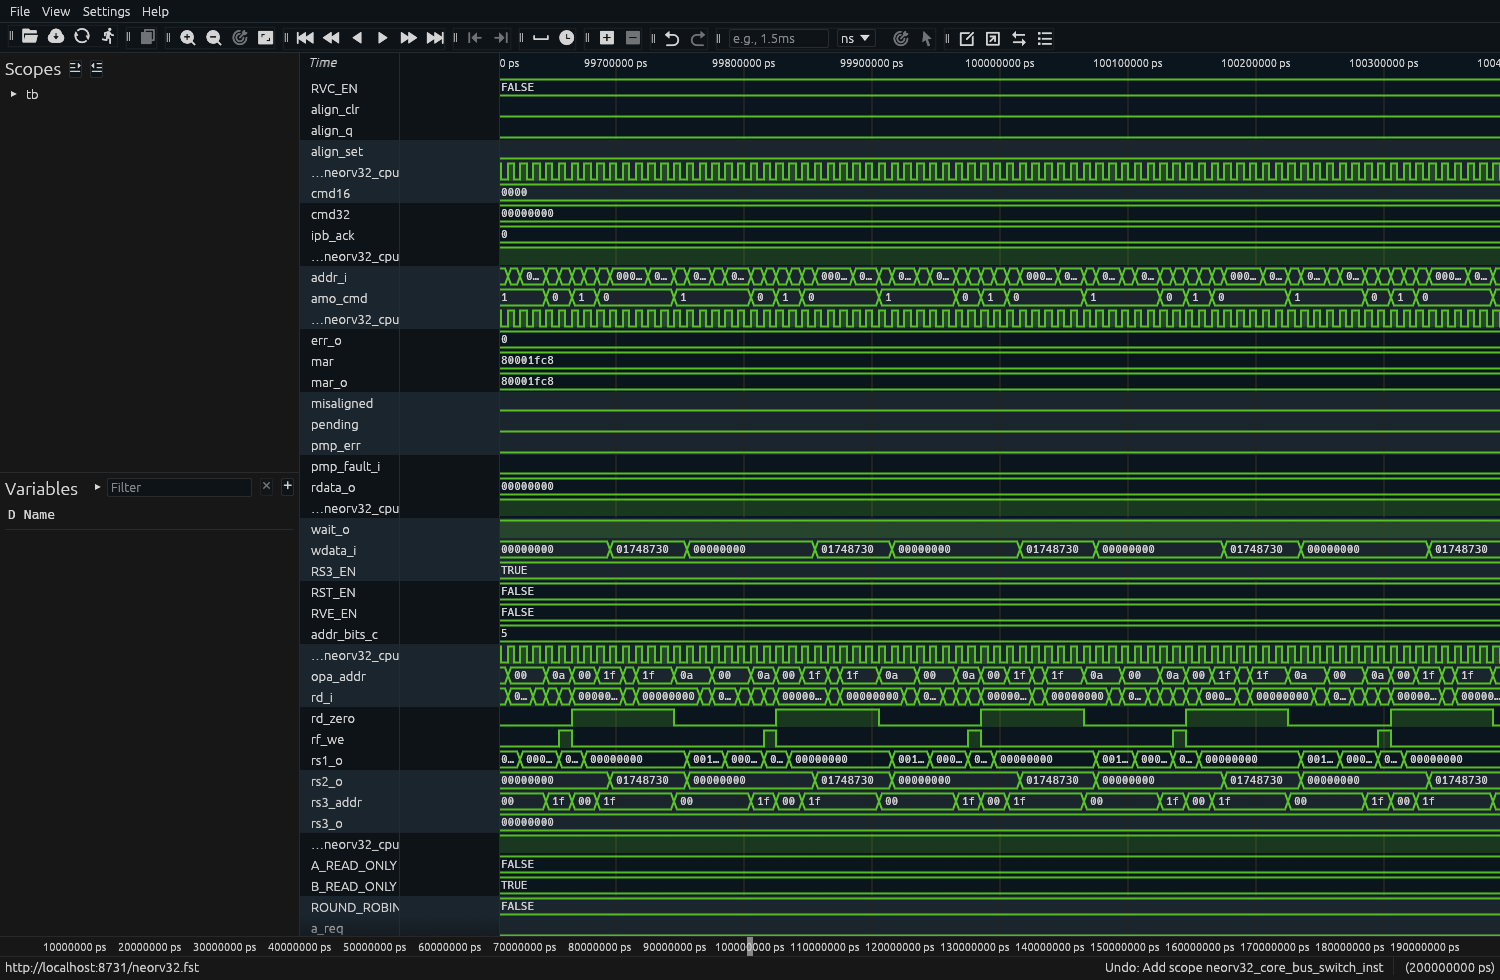
\includegraphics[width=\textwidth]{figures/neorv32-soc-surfer.png}
  \caption{The largest design in the suite after conversion: signals
  from four modules of one NEORV32 core at once, the instruction
  frontend, the load and store unit, the register file and the bus
  switch between them. The database holds 5696 objects in 4832 scopes;
  the rows that read \texttt{TRUE} and \texttt{FALSE} are VHDL
  generics, and the rows that read \texttt{80001fc8} are integers and
  vectors, none of which Vivado's VCD of the same run declares.}
  \label{fig:soc}
\end{figure*}

Fig.~\ref{fig:soc} shows that design after conversion, with signals
from four of its modules on one screen. A design of that size is also
the only kind that exercises the parts of the format a small case
never reaches, which is what the two defects above have in common.

\subsection{A defect found in the checker}

NEORV32 also exposed a limitation in the VCD parser used as guard~2. A
VCD identifier code may be any printable ASCII, and a design with
enough variables receives codes such as \texttt{\#0}, which the
parser's lexer read as a timestamp, and \texttt{R0}, which it read as
a real. The fix, a lexer state in which the word after a value is the
identifier code whatever it looks like, was contributed upstream.

% SPDX-License-Identifier: Apache-2.0
\section{Output: FST through libfst}
\label{sec:output}

\subsection{Why not VCD}

The converter's output format has to hold what the database holds. VCD
does not: the measurement in the introduction, that eight of the
fifteen types in the corpus are absent from Vivado's own VCD, applies
to any VCD. FST~\cite{fst} has variable types for integers, reals,
times and strings, and it compresses far better.

\subsection{Why not a second FST writer}

FST has no standard. The nearest thing to a specification is the
source of \texttt{libfst}~\cite{libfst}, the library GTKWave, GHDL and
nvc all use, plus an unofficial write-up~\cite{hutt}. A second writer
would therefore be a second thing to maintain against a definition
that can move, with nothing to signal that it had drifted.

The converter calls \texttt{libfst} through cgo. The library is three
C source files and zlib, built by Bazel, so the bytes of the output
file come from the reference implementation. The same library reads
the output back in the test.

\subsection{The mapping}

FST has no record type and no array type, so the converter flattens:

\begin{itemize}
  \item a record becomes a scope with one variable per field,
        recursively;
  \item an array of anything but logic becomes a scope with one
        variable per element;
  \item a vector of logic stays one variable of that many bits;
  \item an integer is 32 bits of two's complement, a real is the
        double, and an enumeration, a character, a string or a
        physical value keeps its text.
\end{itemize}

Flattening was chosen so that a viewer can show, search and compare a
single field on its own. The aggregate can be read back from the
leaves; the reverse does not hold.

Two objects that share a handle are declared as one FST variable and
an alias of it, so a signal seen from several scopes is written once.

\subsection{Streaming}

The database stores each object's records where that object's storage
lies, and a waveform file wants every object's changes in ascending
time. The converter therefore replays the file once, keeping the
current value of every object and merging the arenas by record time.
The state is the handle space, 2.8~MB for the largest design here,
rather than the change history, which for that design is
18\,875\,466 entries.

\subsection{Measurements}

\begin{table}[t]
\caption{Conversion, measured on one machine}
\label{tab:cost}
\centering
\begin{tabular}{lrrrr}
\toprule
Design & \texttt{.wdb} & \texttt{.vcd} & \texttt{.fst} & Time \\
\midrule
\texttt{counter} & 14\,kB & 5.6\,kB & 1.6\,kB & 0.02\,s \\
\texttt{uart} & 45\,kB & 3.3\,kB & 2.3\,kB & 0.03\,s \\
PicoRV32 & 268\,kB & 287\,kB & 14\,kB & 0.25\,s \\
Potato & 197\,kB & 28\,kB & 38\,kB & 0.06\,s \\
SERV & 15.9\,MB & 29.6\,MB & 654\,kB & 8.8\,s \\
NEORV32 & 24.1\,MB & 17.2\,MB & 690\,kB & 71\,s \\
\bottomrule
\end{tabular}
\end{table}

Table~\ref{tab:cost} gives the cost. On the two long traces the FST is
45 and 25 times smaller than the VCD of the same run while holding
more. Potato is the instructive row: its FST is larger than its VCD,
because the VCD holds none of that design's integers, enumerations,
records or its two 32\,768 byte memories, and the FST holds all of
them.

Time is dominated by decoding a value and rendering its leaves for
every change, about 3.8~\textmu s per change. Memory is dominated by
holding the inflated pages of the whole database.

% SPDX-License-Identifier: Apache-2.0
\section{Limits}
\label{sec:limitations}

\subsection{One version}

Every claim here was measured on files written by Vivado 2025.2.
Nothing distinguishes a property of the format from a property of that
release, because no second release has been examined. Any use of this
work on another version should begin by re-running the corpus.

\subsection{What is still unexplained}

The repository keeps an open questions section, separate from the
findings table, and it is not short. Among its entries: what the
chunking constants 24 and 299 mean; what several handle space costs
pay for, including the \texttt{0x1088} bytes before the first signal;
which value class codes the corpus has never produced; and what a
numbering added under \texttt{-debug all} is read by. Each is labelled
a guess or a gap. None of them is required by the reader, which is why
they can stay open.

\subsection{The derivation}

An AI agent produced this analysis, under human supervision, by
running experiments and reading bytes. No AMD documentation, source or
binary was used, and the result is not a port, a decompilation or a
specification.

The failure mode of such a derivation is a story that reproduces on
the cases that produced it. The corpus, the truth files, the external
guards and the requirement that every finding name a reproducing
command are all directed at that failure mode. They reduce it; they do
not remove it. Where a wrong answer would be silent and expensive,
the recommendation in the tool's own help text is to open the database
in Vivado instead.

\subsection{Scope of the reader}

The reader decodes the objects a simulation records. It does not
decode the contents of SystemVerilog dynamic objects, which the
database appears to declare and not to record, and it does not write
databases.

% SPDX-License-Identifier: Apache-2.0
\section{Conclusion}

An undocumented binary format was worked out from experiments alone,
to the point where a reader reproduces a declared ground truth for
1049 minimal cases and for six designs, the largest of which records
18\,875\,466 value changes over 5696 objects, and where a converter
produces FST files that a standard viewer opens.

Three parts of the method carried the result. Minimal pairs, so that a
difference between two databases has one cause. A ground truth written
from the design before the database is opened, so that a decoding
claim can fail. And guards outside the project, so that the checker
and the decoder cannot share a mistake.

Two directions remain open. A second Vivado version would separate
properties of the format from properties of one release, which is the
largest single gap in what can be claimed. A large SystemVerilog
design would do for that language what NEORV32 did for VHDL: the
corpus covers SystemVerilog only in miniature, and the two defects
found by large designs were both found in the parts of the format that
only a large design exercises.

\section*{How it is built, and why}

Everything here is built by Bazel: the Vivado installation, every
corpus simulation, the reader, the converter, the C library it calls,
and this report. That is not a preference for a build tool. The method
of Section~\ref{sec:method} rests on a case differing from another
case in one way, so the rest of the environment has to be pinned:
the simulator version, the source files, the compile order, the flags,
and the tool that reads the result. Bazel gives declared inputs,
cached outputs and nothing rebuilt without a reason, which is what
makes a difference between two databases a difference in the design
rather than in the machine that produced it.

The installation is provisioned into a shared cache by
\texttt{rules\_vivado}, so the simulator itself is a build input
rather than something a person installed. The corpus is 1049
simulation targets, and one command re-runs them all. The C library
of Section~\ref{sec:output} is built with a Bazel-fetched toolchain,
so the release binary does not depend on the compiler of the machine
that built it.

The reasoning behind that setup, and the pinning it requires, is
written up on the author's site: hermetic, ephemeral and reproducible
builds~\cite{her}, the whole hardware stack under one build
system~\cite{btd}, an ephemeral machine to run them
on~\cite{homelab}, and the Vivado rules
themselves~\cite{rulesvivado}.

\section*{Availability}

The repository, the corpus, the format documents and the tool are at
\url{https://git.hdlfactory.com/HDL/wdbcvt}. This report is built from
\texttt{//docs/latex} in that repository and is attached to each
release.

The forge is private, and the reason is the runner. A build here needs
a machine with the Vivado installation and the shared caches on it,
because every corpus case is a simulation; a hosted runner cannot do
that. The repository is therefore where the runner is.

If you would like the source in a public place and are willing to
sponsor a runner that can hold a Vivado installation, please get in
touch through \url{https://hdlfactory.com}. That is the one thing
standing between this work and a public mirror.


\balance

\begin{thebibliography}{9}

\bibitem{ieee1800}
IEEE Standard for SystemVerilog, IEEE Std 1800-2023. The VCD format is
defined in its clause on value change dump files.

\bibitem{fst}
T.~Bybell, ``FST file format,'' GTKWave documentation.
\url{https://gtkwave.github.io/gtkwave/internals/fst-file-format.html}

\bibitem{libfst}
GTKWave project, \texttt{libfst}, MIT licensed.
\url{https://github.com/gtkwave/libfst}

\bibitem{hutt}
T.~Hutt, ``An unofficial specification of the FST waveform format.''
\url{https://blog.timhutt.co.uk/fst_spec/}

\bibitem{serv}
O.~Kindgren, ``SERV, the award-winning bit-serial RISC-V core.''
\url{https://github.com/olofk/serv}

\bibitem{potato}
K.~K.~Skordal, ``Potato, a simple RISC-V processor in VHDL.''
\url{https://github.com/skordal/potato}

\bibitem{picorv32}
C.~Wolf \emph{et al.}, ``PicoRV32, a size-optimized RISC-V CPU.''
\url{https://github.com/YosysHQ/picorv32}

\bibitem{neorv32}
S.~Nolting, ``NEORV32, a customizable RISC-V microcontroller.''
\url{https://github.com/stnolting/neorv32}

\bibitem{her}
F.~Filmar, ``Hermetic, ephemeral, reproducible builds.''
\url{https://hdlfactory.com/note/2024/05/01/hermetic-ephemeral-reproducible-builds-her/}

\bibitem{btd}
F.~Filmar, ``Bazel all the way down: how I build programmable
hardware.''
\url{https://hdlfactory.com/post/2026/08/17/bazel-all-the-way-down-how-i-build-programmable-hardware/}

\bibitem{homelab}
F.~Filmar, ``My homelab is fully ephemeral.''
\url{https://hdlfactory.com/post/2026/08/30/fully-ephemeral-homelab/}

\bibitem{rulesvivado}
F.~Filmar, ``rules\_vivado: FPGA synthesis and place-and-route in
Bazel.''
\url{https://hdlfactory.com/post/2026/09/03/rules-vivado-fpga-synthesis-in-bazel/}

\bibitem{ibex}
lowRISC, ``Ibex, a small 32 bit RISC-V CPU core.''
\url{https://github.com/lowRISC/ibex}

\bibitem{govcd}
F.~Filmar, ``go-vcd-parser, a VCD parser and toolkit in Go.''
\url{https://github.com/filmil/go-vcd-parser}

\end{thebibliography}

\end{document}
